\documentclass[12pt]{article}
\usepackage[english]{babel}
\usepackage[utf8x]{inputenc}
%\usepackage[a4paper, total={6in, 8in}]{geometry}
\usepackage[margin=0.5in]{geometry}
\usepackage{graphicx}
\usepackage{subcaption}
\usepackage{placeins}
\renewcommand{\thesubsection}{\thesection.\alph{subsection}}

%-------------- TITLE -----------------%
\author{James Ogle}
\title{ECE414 -- Milestone 2}

%---------- START DOCUMENT ------------%
\begin{document}
\pagenumbering{gobble}
\maketitle
\pagenumbering{arabic}
\section*{Project Overview}
\begin{itemize}
    \item \textbf{Idea:} A rover is placed at a starting position in an unknown grid-based area and is given a goal position to reach.
    The rover must explore partially observed terrain, choose movement directions, and reach the end goal while accounting for obstacles and stochastic movement failures.

    \item \textbf{Current Implementation:} Currently, the environment is setup to where the rover has a "see-able" area which is highlighted in light grey that adjusts as the robot moves.
    A basic reward system has also been setup to provide feedback when the rover has a successful move or not.

    \item \textbf{What Remains:} The next stage will be setting up a policy model to work with the environment (ex. Q-learning).
\end{itemize}

\section*{Environment Design}
\begin{itemize}
    \item \textbf{Environment:} The environment is an $11 \times 11$ grid-based lunar surface containing boundary walls, randomly generated obstacle terrain, a rover start position at $(1,1)$, and a goal beacon at $(9,9)$.
    Breadth-first search verifies that a valid path from the start to the goal exists before each episode begins. The rover initially observes only a local region around its position, while the rest of the terrain remains unknown.

    \item \textbf{State/Observation:} The rover receives a partially observable MiniGrid observation after each action.
    This observation contains a local encoded view of nearby cells, the rover's facing direction, and the mission text; it does not provide the full map or all obstacle locations.
    Internally, the environment tracks the rover position, goal position, discovered cells, and the hidden grid layout.

    \item \textbf{Action:} The agent selects one of four discrete actions: move east, south, west, or north.
    These actions are encoded as $0$, $1$, $2$, and $3$, respectively.

    \item \textbf{Reward:} The agent receives a small step penalty of $-0.01$ to encourage efficient movement.
    It receives $+0.02$ for each newly revealed cell, $+1.0$ for reaching the goal, $-0.05$ for attempting to enter an obstacle or wall, and an additional $-0.25$ if a stochastic movement failure occurs.

    \item \textbf{Transition:} After the rover selects a direction, the environment checks the adjacent target cell.
    If the cell is a wall or obstacle, the rover remains in its current position; otherwise, it moves to that cell unless a random movement failure occurs, which has a probability of $0.15$.
    After the transition, nearby cells are marked as discovered, a new partial observation is returned, and the episode terminates when the rover reaches the goal or is truncated after the maximum number of steps.
\end{itemize}
\clearpage
\begin{figure}[htbp]
    \centering
    \begin{subfigure}[t]{0.48\textwidth}
        \centering
        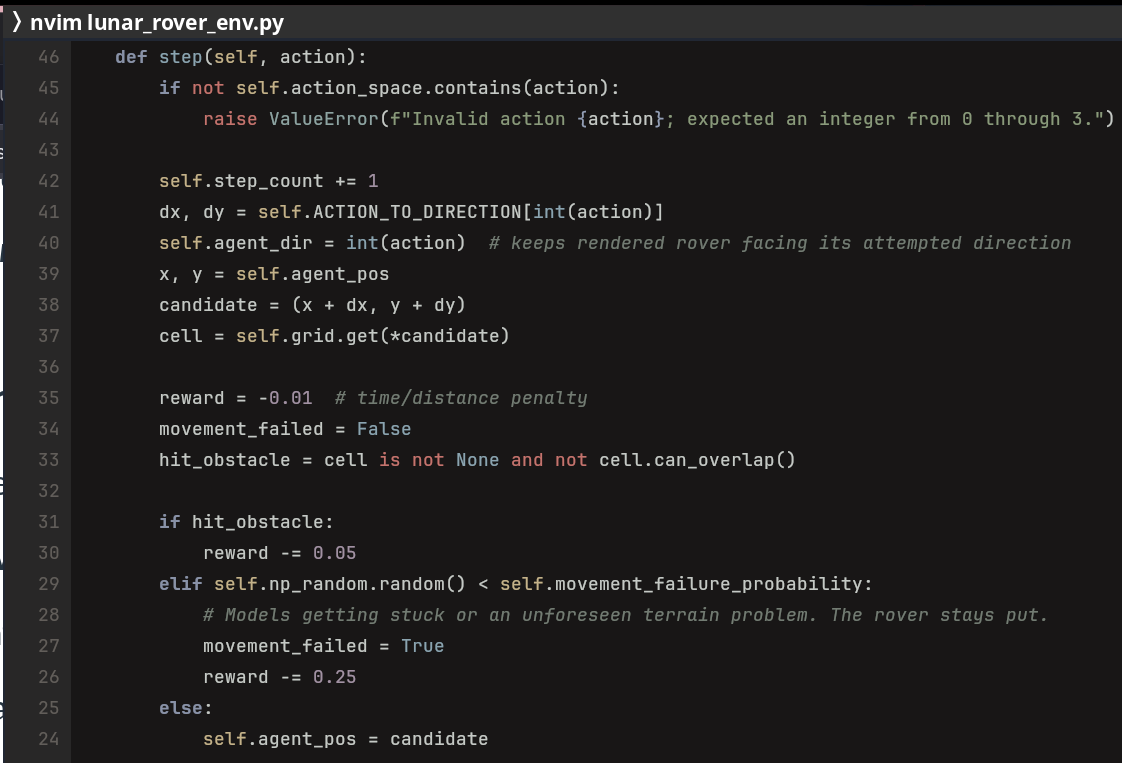
\includegraphics[width=\textwidth]{./img/step_1.png}
        \caption{First Part of step function in environment}
        \label{fig:left}
    \end{subfigure}
    \begin{subfigure}[t]{0.48\textwidth}
        \centering
        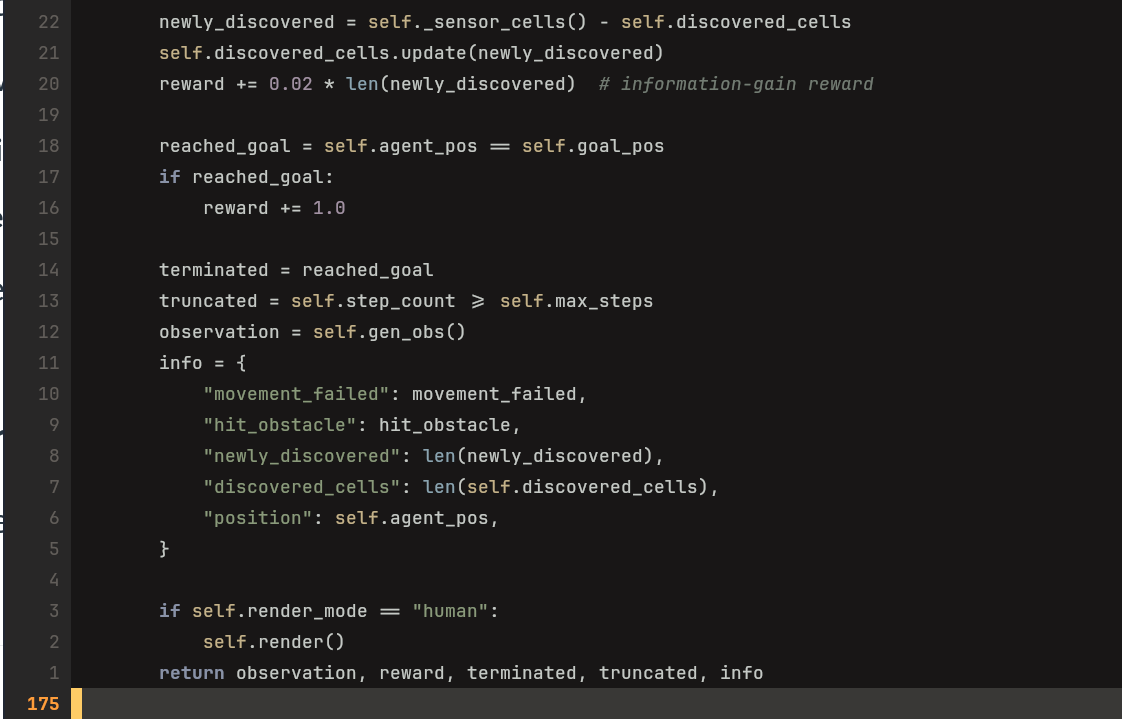
\includegraphics[width=\textwidth]{./img/step_2.png}
        \caption{Second Part of step function in environment}
        \label{fig:right}
    \end{subfigure}
\end{figure}

\noindent The code above is the step method of environment class split up into two pictures.
The method updates the step-count, applies reward values, and setups new observation information for the next step.
The method will also determine if the episode needs to halt or not whether that is from reaching the end goal or the allotted amount of steps setup by the user.
\begin{figure}[htbp]
    \centering
    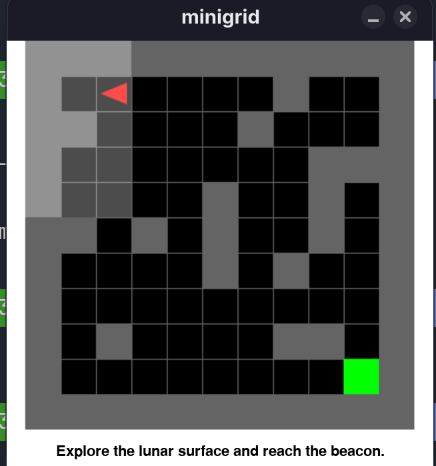
\includegraphics[width=0.48\textwidth]{./img/image_of_grid.png}
    \caption{Rendered Lunar Rover environment after initialization. The red rover begins near the upper-left area, the green cell is the goal beacon, black cells are obstacle terrain, and the gray highlighted region represents the rover's local observable area.}
\end{figure}

\FloatBarrier

\section*{Environment Testing}
\begin{itemize}
    \item \textbf{Testing Environment:} I tested the environment by running \texttt{lunar\_rover\_env.py},
    which creates a \texttt{LunarRoverEnv} instance, calls \texttt{reset(seed=7)}, and executes 25 randomly sampled actions.
    During the test, the environment prints the selected action, reward, rover position, number of discovered cells, collision status, and whether stochastic movement failure occurred.
    I also visually inspected the rendered MiniGrid window to confirm that walls, obstacles, the rover, and the goal were displayed correctly.

    \item \textbf{Environment Response to Agent Action:} For each action, the \texttt{step()} method converts the selected value into one of four cardinal directions.
    A valid move changes the rover position; an attempted move into a wall or obstacle leaves it in place and applies a collision penalty.
    Even valid moves can fail with probability $0.15$, representing the rover becoming stuck or encountering unknown terrain.
    The environment then returns the next partial observation, reward, termination flags, and diagnostic information.

    \item \textbf{Correctly Initializing Environment:} The \texttt{reset()} method regenerates the grid, places the rover at the fixed start position $(1,1)$, places the goal at $(9,9)$ for the default $11 \times 11$ grid, and initializes the set of discovered cells around the rover.
    Obstacle positions are randomly generated, but breadth-first search verifies that at least one path from the start to the goal exists before the episode begins.
    Using the same seed reproduces the same randomly generated environment for debugging.

    \item \textbf{Technical Challenges/Constraints:} A main challenge was generating random obstacle layouts without producing impossible episodes.
    This was addressed by using breadth-first search during grid generation to reject layouts without a valid start-to-goal path.
    Another constraint is partial observability: the rover receives a local MiniGrid observation instead of the entire grid.
    Finally, stochastic movement introduces uncertainty because a valid action may fail even when the selected cell is reachable.
\end{itemize}

% Figure 3: testing evidence
\begin{figure}[htbp]
    \centering
    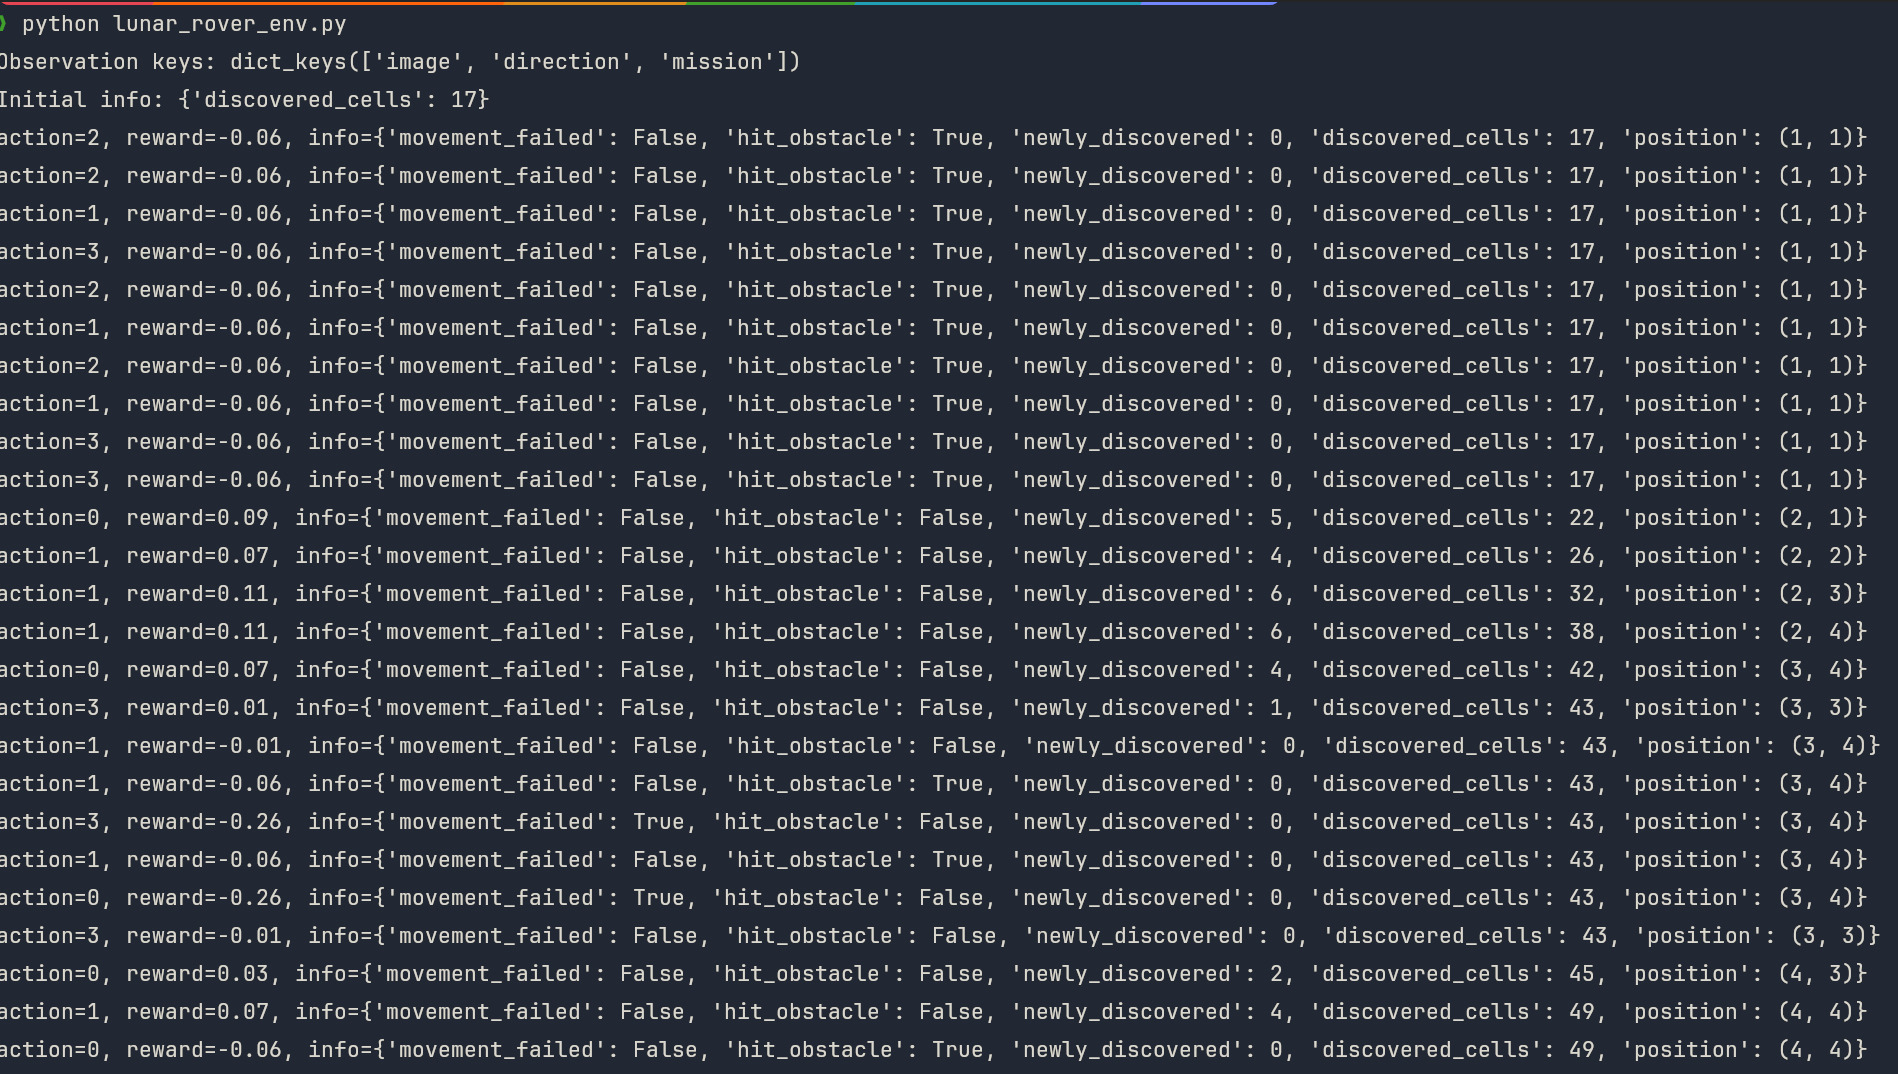
\includegraphics[width=0.82\textwidth]{./img/test_run_output.png}
    \caption{Sample output from testing the Lunar Rover environment.
    Each line reports an action, reward, rover position, and transition
    information returned by \texttt{step()}.}
    \label{fig:test-output}
\end{figure}

\section*{Next Steps}
The next step is to implement a tabular Q-learning policy and train it through repeated interactions with the Lunar Rover environment.
The agent will learn action values for observed states using the rewards and transition outcomes implemented in this milestone.
\bigskip

A current challenge will be designing a state representation that allows the agent to distinguish newly explored terrain from previously visited terrain.
The exploration reward and an epsilon-greedy action-selection policy will be used to reduce repeated movement through already explored cells and improve progress toward the goal.
\end{document}
